% Created 2021-01-24 Sun 22:50
% Intended LaTeX compiler: pdflatex
\documentclass[11pt]{article}
\usepackage[utf8]{inputenc}
\usepackage[T1]{fontenc}
\usepackage{graphicx}
\usepackage{grffile}
\usepackage{longtable}
\usepackage{wrapfig}
\usepackage{rotating}
\usepackage[normalem]{ulem}
\usepackage{amsmath}
\usepackage{textcomp}
\usepackage{amssymb}
\usepackage{capt-of}
\usepackage{hyperref}
\usepackage{minted}
\hypersetup{colorlinks=true, linkcolor=black, filecolor=red, urlcolor=blue}
\usepackage[turkish]{babel}
\author{Eren Hatırnaz}
\date{1 Eylül 2019}
\title{Yazılım Gündemi - 7\\\medskip
\large 26 Ağustos - 1 Eylül 2019}
\hypersetup{
 pdfauthor={Eren Hatırnaz},
 pdftitle={Yazılım Gündemi - 7},
 pdfkeywords={},
 pdfsubject={},
 pdfcreator={Emacs 27.1 (Org mode 9.3)},
 pdflang={Turkish}}
\begin{document}

\maketitle
\tableofcontents \clearpage\shorthandoff{=}

\begin{center}
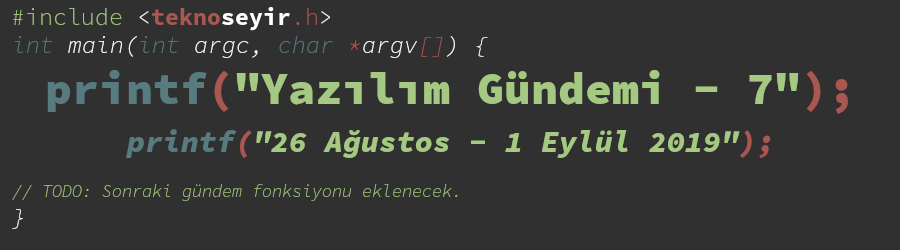
\includegraphics[width=.9\linewidth]{gorseller/yazilim-gundemi-banner.png}
\end{center}

\begin{center}
\href{../06/yazilim-gundemi-06.pdf}{< Önceki Gündem} | \textbf{26 Ağustos - 1 Eylül 2019} | \href{../08/yazilim-gundemi-08.pdf}{Sonraki Gündem >}

\href{https://teknoseyir.com/blog/yazilim-gundemi-7-26-agustos-1-eylul-2019}{TeknoSeyir'de Oku}
\end{center}

\section{PHP Central Europe konferansı \href{https://www.theregister.co.uk/2019/08/27/php\_europe\_cancelled/}{cinsiyetçilik suçlamaları yüzünden iptal edildi}}
\label{sec:org1268ad3}
PHP topluluğundaki büyük organizasyonlardan biri olan PHP CE, bu yıl Almanya'da
gerçekleşmesi planlanan etkinliğin \href{http://2019.phpce.eu/en/}{web sitesinin ana sayfası}nda kısa bir mesaj
yayınlayarak, konferansın iptal edildiğini ve devam etmeyeceğini duyurdu.
Konferansın iptal edilme sebebi olarak da dipnot olarak şu üç tweet
paylaşımının bağlantısını vermişler:

\begin{itemize}
\item \href{https://twitter.com/KarlLHughes/status/1151525811616387073}{Tweet 1}
\item \href{https://twitter.com/Crell/status/1152368497823031296}{Tweet 2}
\item \href{https://twitter.com/Mark\_Baker/status/1154113051056099329}{Tweet 3}
\end{itemize}

Olayları özetlemek gerekirse: Organizatörler normal işleyişe uygun olarak
geçtiğimiz aylarda Konuşmacı Çağrısı (Call for Proposals) yapmışlar. Çağrı
süresi bitince de, gelen başvurular içerisinden konferans içeriğine uygun
olanları seçmişler ve geçtiğimiz haftalarda da konuşmacı listesi yayınlanmış.

Olaylar da burdan sonra başlıyor zaten. Yukarıdaki ilk tweet'de başlangıç
ateşini sağlamış. Konferansın "tamamen beyaz erkek konuşmacılar"dan oluştuğunu
söylemiş ve utanç duyduğunu belirtmiş. Tweet altında bir sürü tartışma mevcut.

Diğer tweet iki tweet blog yazılarının duyurusundan ibaret. Larry Garfield
tarafından yazıyı kısaca özetlemek gerekirse: Bu yılın başlarında PHP CE
organizatörleri kendisine konferansta konuşmacı olmayı teklif etmişler ve kabul
etmiş. Konuşmacı listesi açıklandıktan sonra hiç kadın konuşmacı olmamasından
dolayı bir rahatsızlık duymuş ve konuyu organizatörler ile konuşarak, gerekirse
konuşmacı bulma ve masrafları karşılama konusunda yardımcı olabileceğini
söylemiş. Organizatörler, "böyle bir düzenlemeye açık olmadıklarını"
belirtmişler ve gelen başvurulardan sadece bir tanesinin kadın olduğunu, onun
da daha önce lokal bir etkinlikle yapılan sunumun tekrarı olduğu için
reddedildiğini söylemişler. Anladığım kadarıyla bu kişi organizatörler ile
konuşmacı başvurusu süreci dolduktan sonra konuşmuş. Zaten yazıda da
organizatörlerin "konuşmacı çağrısı süreci doldu ve yeniden açamayız"
dediklerini aktarıyor. Bunun üzerine blog yazısını yazan kişi de etkinlikte
konuşmacı olmaktan vazgeçtiğini söylüyor.

Diğer blog yazısında da Mark Baker isimli kişi etkinlikte konuşmacı olmaktan
aynı nedenlerle vazgeçtiğini söylüyor.

Konu \href{https://www.reddit.com/r/programming/comments/cvtx3w/php\_central\_europe\_conference\_cancelled\_because/}{Reddit} ve \href{https://news.ycombinator.com/item?id=20795709}{HackerNews} gibi platformlarda da bir gün boyunca üst sıralarda
yer aldı ve tartışıldı. Oralarda yazılanların da bazılarını okudum. Benim şahsi
görüşüm pek cinsiyetçi bir tutum olmadığı yönünde. Konuşmacı başvuruları
sürecinin herkes için eşit olması gerektiğini düşünüyorum fakat Larry Garfield
isimli kişiye konuşmacı olmasını teklif etmeleri biraz soru işareti yarattı
bende. Neyse konu hakkında düşünmeye devam edeceğim ben, henüz net bir görüşe
sahip değilim. Siz ne düşünüyorsunuz konu hakkında? Yorumlar kısmında
konuşalım.

Bu arada konuyla ilgili sadece benim yazdıklarımla kalmayıp, ilgili
bağlantılardaki yazıları kendinizin de okumasını tavsiye ederim. Belki benim
yanlış anladığım ya da iyi çeviremediğim kısımları olmuş olabilir, insanları
yanlış yönlendirmek istemem kesinlikle. Lütfen fikir sahibi olmadan önce diğer
yazılanları da okuyun.

Konuyla ilgili, yazılım sektöründe çalışan bir kız arkadaşıma fikirlerini
sordum. Müsait olduğunda yazıları okuyup geri dönüş yapacak. O geri dönüş
yaptığında, onun da görüşlerini buraya ekleyeceğim.
\section{NPM paket yönetim sistemi, terminal çıktısında \href{https://www.zdnet.com/article/npm-bans-terminal-ads/}{reklam göstermeyi yasakladı}}
\label{sec:orgbb24a08}
Geçtiğimiz haftanın Yazılım Gündemi yazısında (bkz: \href{../06/yazilim-gundemi-06.pdf}{Yazılım Gündemi - 6})
bahsetiğim olayın üzerine NPM şirketi \href{https://www.npmjs.com/policies/open-source-terms\#commercial-content}{sözleşmelere} yeni maddeler ekleyerek söz
konusu davranışı da içerisinde barındıran birkaç durumu yasakladı. Bunlar şu
şekilde:

\begin{itemize}
\item Yazılım geliştirme döngüsünün herhangi bir parçasında (çalışma zamanı,
yüklenme vb.) npm betiklerini kullanarak reklam gösteren paketler
yasaklandı.
\item Reklam göstermek için kod parçaları içeren paketlerde sorun yok (büyük
ihtimal siteye reklam eklemeye yarayan yardımcı araçlar kast edilmiş)
fakat doğrudan reklam gösteren paketler yasaklandı.
\item Esas olarak reklam gösteren fakat önemsiz kod, veri ya da diğer teknik
içerikler içeren paketler yasaklandı.
\end{itemize}

\begin{center}
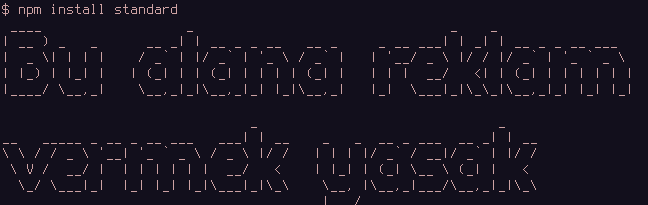
\includegraphics[width=.9\linewidth]{gorseller/reklam-yasak.png}
\end{center}

Bunun üzerine konunun gündeme gelmesini sağlayan kişide detaylıca bir blog
yazısı yazarak olayın nereden başladığını, sürecin nasıl geliştiğini vb. tüm
detaylarını anlattı. İlgili blog yazısına \href{https://feross.org/funding-experiment-recap/}{buradan} ulaşabilirsiniz. Şahsen benim
okuma fırsatım olmadı fakat konuyla ilgilenenlerin mutlaka okuması gereken bir
yazı.

NPM şirketi de kendi blog sitelerinde "\href{https://blog.npmjs.org/post/187382017885/supporting-open-source-maintainers}{Supporting Open Source Maintainers}"
konulu bir yazı yayınlayarak, açık kaynak geliştiricilere destek olmakla ilgili
çalışmalarından bahsetmiş.
\section{Windows Terminal \href{https://devblogs.microsoft.com/commandline/windows-terminal-preview-v0-4-release/}{Preview v0.4 yayınlandı}}
\label{sec:org2168e67}
\begin{center}
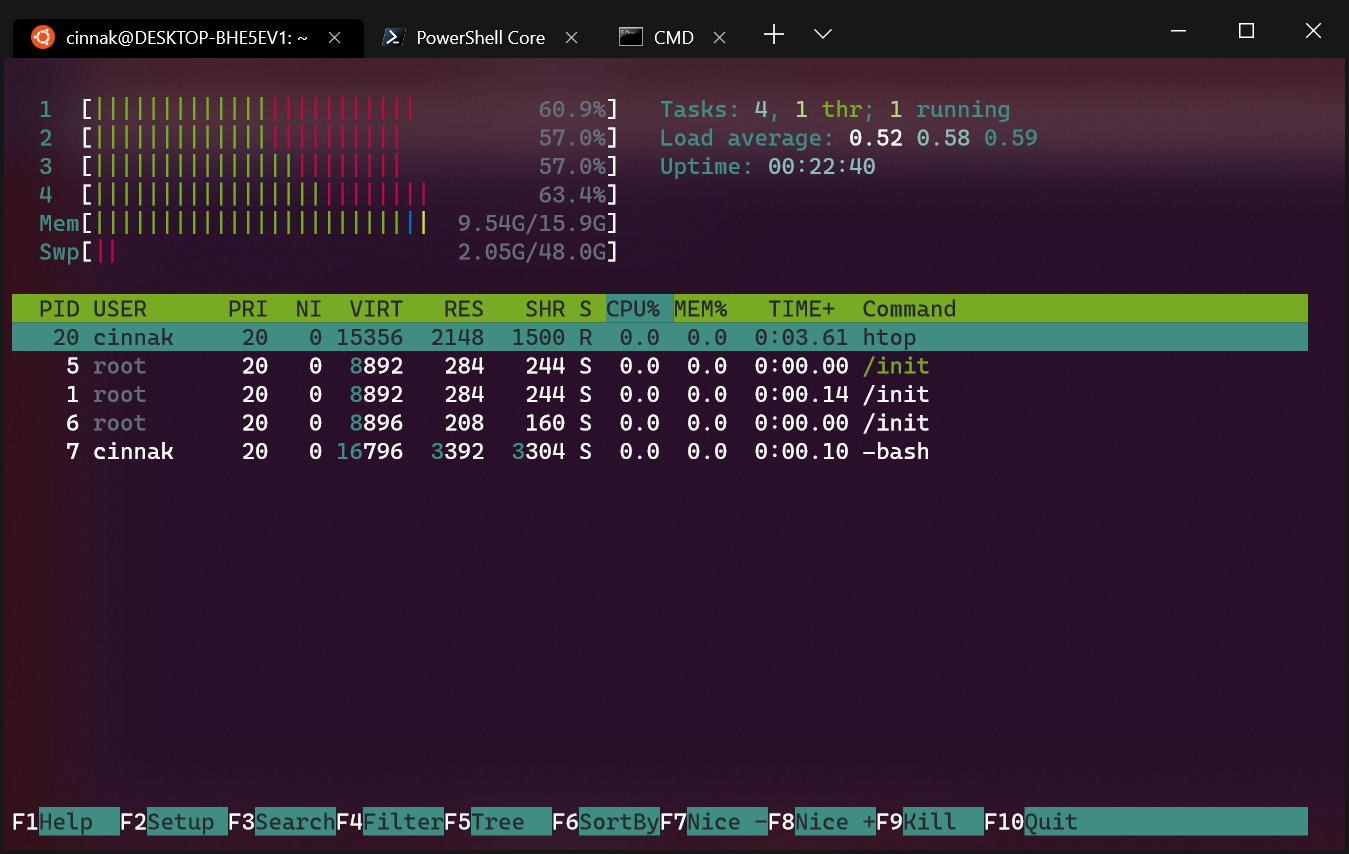
\includegraphics[width=.9\linewidth]{gorseller/windows-terminal-v0_4.png}
\end{center}

Önceki bir yazılım gündemi yazısında da (bkz: \href{../04/yazilim-gundemi-04.pdf}{Yazılım Gündemi - 4}) söylediğim
gibi Microsoft, uzun zamandır kendinden uzaklaşan geliştirici camiasını tekrar
kazanmak için hamleler yapıyor. Bunlardan birisi de Windows Terminal. Bu hafta
bir blog yazısı yayınlayarak preview v0.4 sürümünü duyurdu. Yapılan bazı
değişiklikler şu şekilde:

\begin{itemize}
\item Sekme başlığında artık varsayılan olarak dosya yolu yerine profil ismi
gözükecekmiş fakat isteyenler "tabTitle" özelliğini kendilerine göre
özelleştirebilecek.
\item Terminal uygulamasının ayar dosyasında yanlış bir yer varsa hata gösterecek.
\item Seçileni otomatik kopyalama özelliğiyle ilgili global bir ayar eklenmiş.
\end{itemize}

Diğer değişiklikler için konu başlığına eklediğim blog yazısına göz
atabilirsiniz.

\section{Google, Chrome tarayıcısına, web sitelerinin \href{https://www.techrepublic.com/article/google-moves-closer-to-letting-chrome-web-apps-edit-your-files-despite-warning-it-could-be-abused-in-terrible-ways/}{dosya sistemimize erişmesini sağlayacak API sistemi ekliyor}}
\label{sec:orga7a90d0}
Evet, yanlış okumadınız. İlk gördüğüm de ben de "nasıl ya?" dedim fakat Chrome
ekibi çoktan çalışmalara başlamış ve Chrome 78 sürümünde \href{https://developers.google.com/web/updates/2019/08/native-file-system}{bu özelliği duyurmayı
planlamışlar}. API sisteminin detaylarını pek fazla inceleyemedim ama sadece
https uzantılı sitelerde çalışacağı haberde söylenmiş. Ayrıca \texttt{chrome://flags}
kısmından açıp kapatma opsiyonu da var gözüküyor. Her ne kadar kullanıcı izini
gerektiriyor olsa da bence çok tehlikeli bir sistem. Deneyimli olmayan
kullanıcıların kandırılması ve sistemin suistimal edilmesi çok olası bir durum.
\section{Yeni bir platform girişimi: \href{https://acikkaynakplatformu.github.io/}{Türkiye Açık Kaynak Platformu}}
\label{sec:org4814097}
Sektörden sosyal medya vasıtasıyla tanıdığım birçok isim bir araya gelmişler.
Platform için uzun zamandır toplantılar devam ediyormuş. Bakalım ortaya ne
çıkacak, ben de meraklıyım.

\begin{itemize}
\item \href{https://twitter.com/fkadev/status/1167076567366942720}{Konuyla ilgili tweet}
\end{itemize}
\section{Diğer Haberler}
\label{sec:org067a313}
\begin{itemize}
\item React takımı, ırkçılık suçlamaları nedeniyle \href{https://www.businessinsider.com/reactgate-react-facebook-code-of-conduct-twitter-2019-8}{yeni davranış kuralları
getirmeye hazırlanıyor}.
\item Google, bir geliştiricinin 10 yıllık uygulamasını marketten silmiş fakat
sonra geri adım atmış. Tüm süreç \href{https://medium.com/mmathieum/google-just-deleted-my-nearly-10-year-old-free-open-source-android-app-7fbc52edc50a}{geliştiricinin blog yazısı}nda anlatılmış.
\item Google, veri doğrulama dili \href{https://cuelang.org}{CUE ve araç setini duyurdu}.
\item WMware, Kubernetes sistemiyle ilgili ücretsiz materyal ve derslerin
bulunduğu \href{https://blogs.vmware.com/cloudnative/2019/08/27/introducing-kubernetes-academy-free-cloud-native-education-platform/}{yeni bir platform açtı}: \href{https://kubernetes.academy/}{Kubernetes Acedemy}.
\item Go modülleri için \href{https://blog.golang.org/module-mirror-launch}{index ve checksum veritabanı duyuruldu}.
\item PowerShell içerisine zincir operatörleri \href{https://github.com/PowerShell/PowerShell/pull/9849}{eklenmesi konuşuluyor}.
\item Firefox 70 sürümünde daha hızlı bir \href{https://hacks.mozilla.org/2019/08/the-baseline-interpreter-a-faster-js-interpreter-in-firefox-70/}{JavaScript interpreter gelecekmiş}.
\item TypeScript \href{https://devblogs.microsoft.com/typescript/announcing-typescript-3-6/\#stricter-generators}{3.6 sürümü duyuruldu}.
\item Bir güvenlik açığını kapatan 3 yeni Ruby sürümü yayınlandı:
\begin{itemize}
\item \href{https://www.ruby-lang.org/en/news/2019/08/28/ruby-2-6-4-released/}{2.6.4}
\item \href{https://www.ruby-lang.org/en/news/2019/08/28/ruby-2-5-6-released/}{2.5.6}
\item \href{https://www.ruby-lang.org/en/news/2019/08/28/ruby-2-4-7-released/}{2.4.7}
\end{itemize}
\item Perl topluluğu, \href{https://github.com/perl6/problem-solving/issues/81}{"Perl 6" ismi hakkında tartışıyor}.
\item Julia programlama dili geliştirilmesi ile ilgili durum raporu yayınlandı:
\href{https://julialang.org/blog/2019/08/release-process}{Julia's Release Process}.
\item HHVM 4.20.0 ve 4.20.1 \href{https://hhvm.com/blog/2019/08/27/hhvm-4.20.0.html}{sürümleri duyuruldu}.
\item Dağıtık şekilde SQLite veritabanları barındırmaya yarayan \href{https://dqlite.io/}{Dqlite} aracının
\href{https://github.com/canonical/dqlite/releases/tag/v1.0.0}{ilk stabil sürümü duyuruldu}.
\item Postgres üzerinde WebAssembly çalıştırmaya yarayan eklenti \href{https://medium.com/wasmer/announcing-the-first-postgres-extension-to-run-webassembly-561af2cfcb1}{açık kaynak
olarak yayınlandı}: \href{https://github.com/wasmerio/postgres-ext-wasm}{postgres-ext-wasm}.
\item Emacs \href{https://lists.gnu.org/archive/html/emacs-devel/2019-08/msg00577.html}{26.3 yayınlandı}.
\item Emacs org-mode için sorgu dili kütüphanesi org-ql, \href{https://github.com/alphapapa/org-ql\#02}{v0.2 sürümünü duyurdu}.
\item Bilgisayara bağlı cihazlar ile iletişim kurmayı sağlayan \href{https://github.com/MelbourneDeveloper/Device.Net}{Device.Net}
kütüphanesi \href{https://christianfindlay.com/2019/08/26/device-net-3-0/}{3.0 sürümünü duyurdu}. \href{https://github.com/MelbourneDeveloper/Device.Net/projects/8}{Değişiklik Notları}.
\item \href{https://timothycrosley.github.io/portray/}{Portray} isimli Python projelerinizin dokümantasyonu için web sitesi
oluşturma aracı \href{https://timothycrosley.github.io/portray/CHANGELOG/}{ilk stabil versiyonunu yayınlandı}.
\item Test ve prototipleme için kullanılmak üzere sahte bilgiler döndüren GraphQL
API sistemi açık kaynak olarak yayınlandı: \href{https://graphqlzero.almansi.me/}{GraphQLZero}, \href{https://github.com/ealmansi/gqlz}{GitHub Deposu}.
\item Dağıtık PGP anahtar sunucusu projesi \href{https://github.com/tdjsnelling/dat-keyserver}{dat-keyserver}, \href{https://github.com/tdjsnelling/dat-keyserver/releases/tag/v1.5.0}{v1.5.0 sürümünü} çıkardı.
\item Oyun programlama için kullanılan C++ kütüphanesi EnTT, \href{https://github.com/skypjack/entt/releases/tag/v3.1.0}{v3.1.0 sürümünü duyurdu}.
\item Güvenli gömülü sistemler inşa etmek için ADA dili ile geliştirilen
microkernel \href{https://wookey-project.github.io/ewok/index.html}{EwoK}, \href{https://github.com/wookey-project/ewok-kernel/releases/tag/v0.9.9}{v0.9.9 sürümünü çıkardı}.
\item Firebase için ORM aracı olan firebase-firestorm, \href{https://github.com/lmcq/firebase-firestorm/releases/tag/v1.1.0}{v1.1.0 sürümünü çıkardı}.
\item Log kayıtlarını çeşitli servislere göndermeye yarayan PHP kütüphanesi
monolog, \href{https://github.com/Seldaek/monolog/releases/tag/2.0.0}{v2.0.0 sürümü duyurdu}.
\item Google Summer of Code projesi \href{https://lists.freedesktop.org/archives/wayland-devel/2019-August/040819.html}{Waypipe tamamlandı}, \href{https://gitlab.freedesktop.org/mstoeckl/waypipe/}{GitLab Deposu}.
\item JOOQ, \href{https://blog.jooq.org/2019/08/29/jooq-3-12-released-with-a-new-procedural-language-api/}{3.12 sürümünü duyurdu}.
\item etcd, \href{https://kubernetes.io/blog/2019/08/30/announcing-etcd-3-4/}{3.4 sürümü duyuruldu}.
\end{itemize}
\section{Lisans}
\label{sec:org3b731ad}
\begin{center}
\begin{center}

\includegraphics[height=1.5cm]{../../../img/CC_BY-NC-SA_4.0.png}
\end{center}

\href{yazilim-gundemi-07.pdf}{Yazılım Gündemi - 7} yazısı \href{https://erenhatirnaz.github.io}{Eren Hatırnaz} tarafından \href{http://creativecommons.org/licenses/by-nc-sa/4.0/}{Creative Commons
Atıf-GayriTicari-AynıLisanslaPaylaş 4.0 Uluslararası Lisansı} (CC BY-NC-SA 4.0)
ile lisanslanmıştır.
\end{center}
\end{document}
